\chapter{Metodologia}
\label{cap:metodologia}
Este capítulo apresenta o detalhamento do desenvolvimento do sistema proposto, dividido em três subprocessos principais: a configuração da prova, a correção geral da prova e a correção específica das respostas que exigem intervenção adicional. Cada subprocesso será explicado detalhadamente utilizando fluxogramas para ilustrar os passos realizados. A seguir são apresentados os fluxogramas que ilustram cada um dos subprocessos mencionados (Figuras
\autoref{fig:fluxo-configuracao},
\autoref{fig:fluxo-correcao-prova} e
\autoref{fig:fluxo-correcao-pergunta}).


\begin{figure}[H]
    \centering
    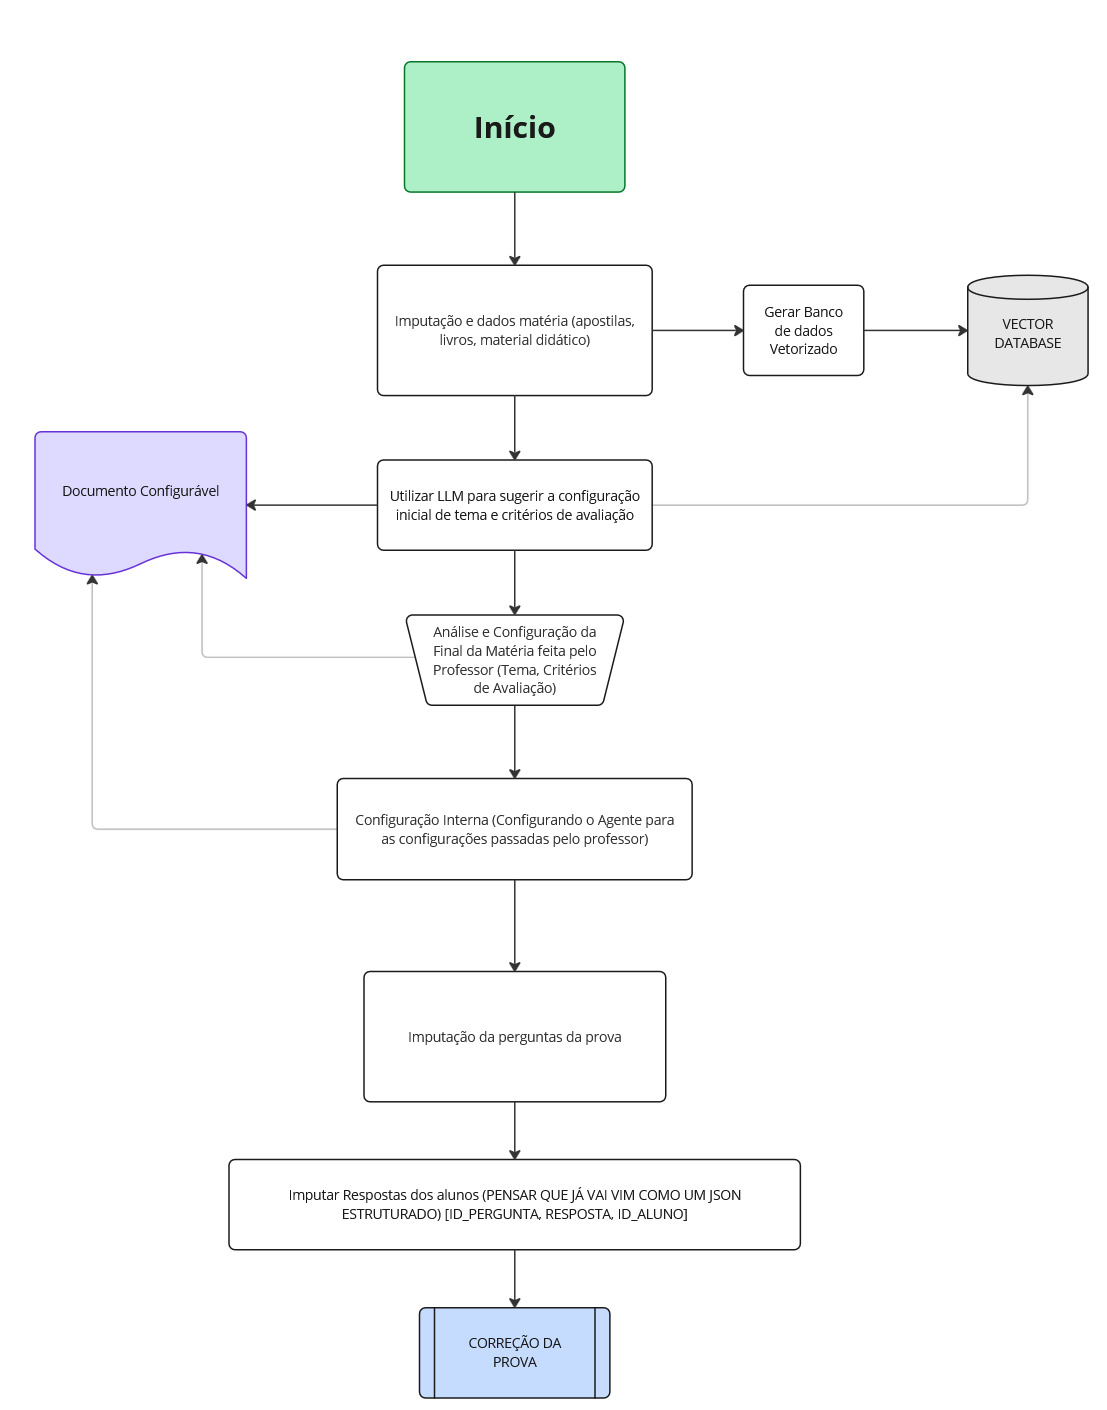
\includegraphics[width=\textwidth]{media/fluxo-configuracao.jpg}
    \caption{Fluxograma do subprocesso de configuração da prova}
    \label{fig:fluxo-configuracao}
\end{figure}

\begin{figure}[H]
    \centering
    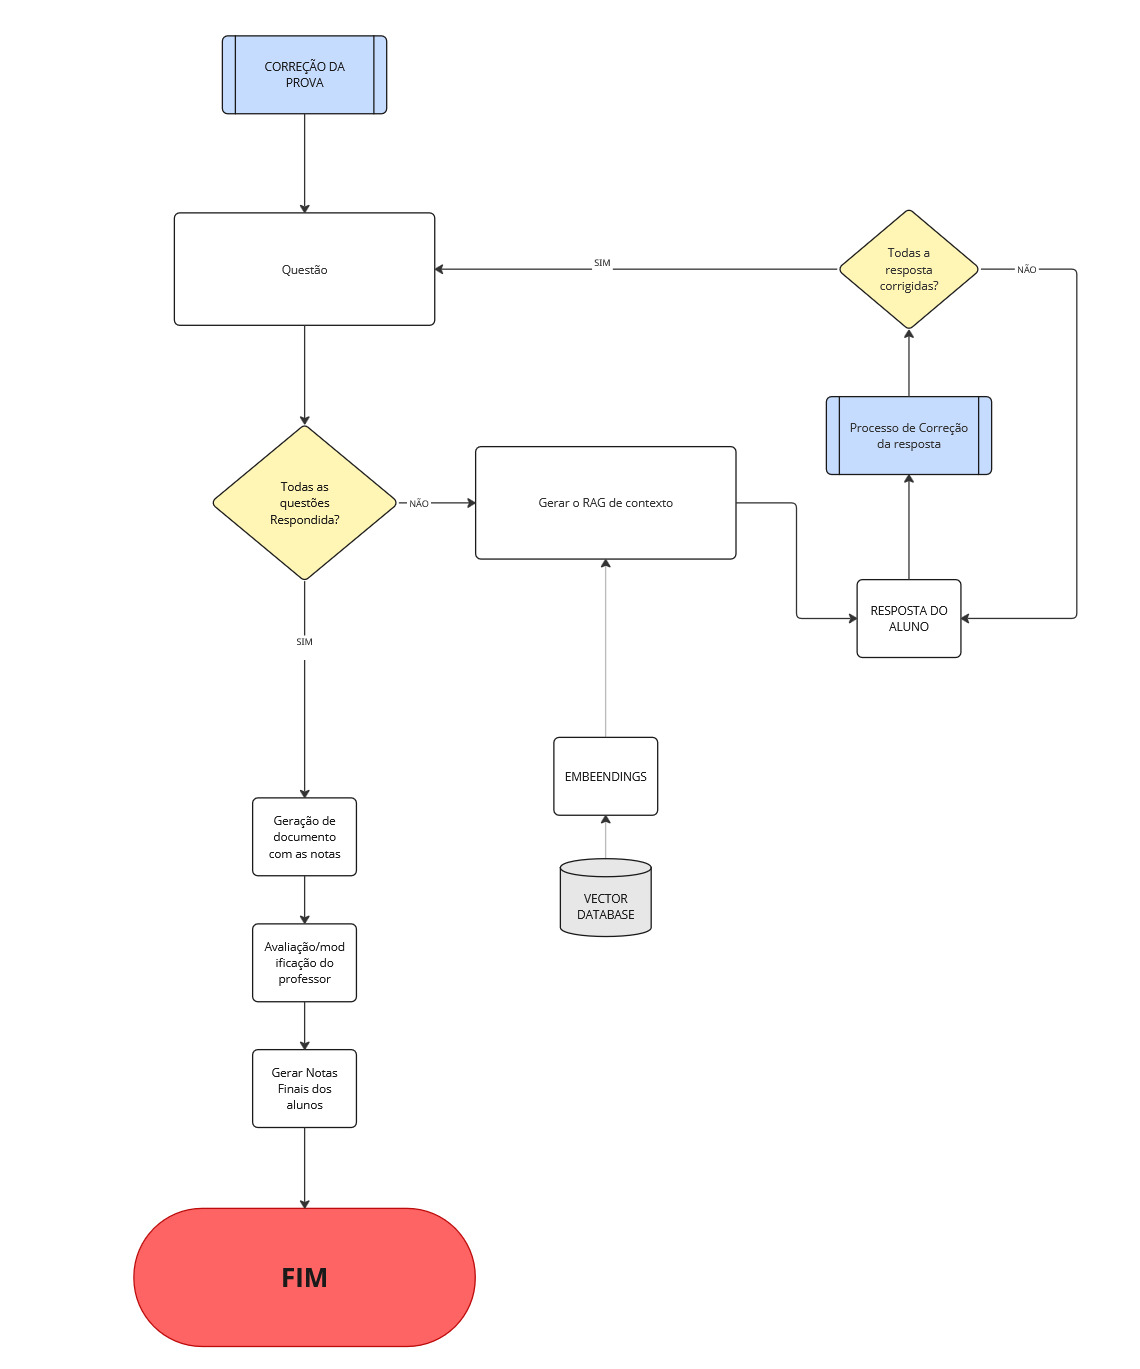
\includegraphics[width=\textwidth]{media/fluxo-correcao-prova.jpg}
    \caption{Fluxograma do subprocesso de correção da prova}
    \label{fig:fluxo-correcao-prova}
\end{figure}

\begin{figure}[H]
    \centering
    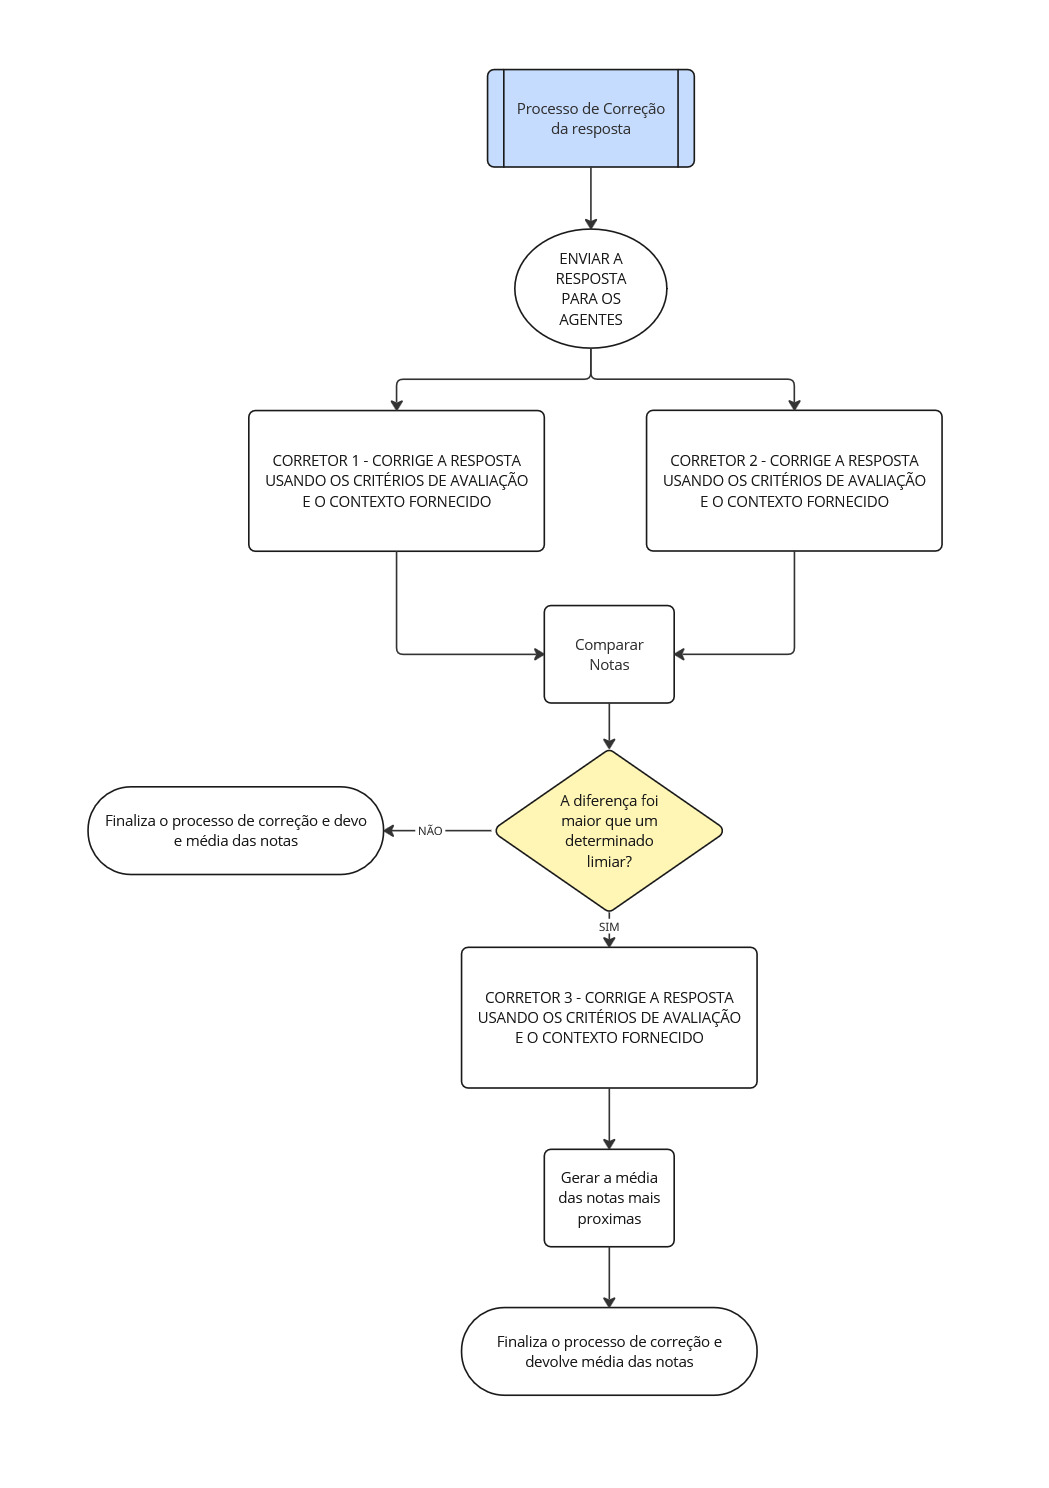
\includegraphics[width=\textwidth]{media/fluxo-correcao-pergunta.jpg}
    \caption{Fluxograma do subprocesso de correção da resposta}
    \label{fig:fluxo-correcao-pergunta}
\end{figure}


\section{Subprocesso de Configuração da Prova}

O subprocesso de configuração da prova é iniciado com a coleta e imputação dos materiais didáticos (apostilas, livros, entre outros) utilizados como base para a formulação das questões. Posteriormente, esses materiais são vetorizados e armazenados em um banco de dados vetorial (\textit{Vector Database}).

Uma LLM sugere então uma configuração inicial baseada nos critérios gerais estabelecidos. Essas sugestões são revisadas e refinadas pelo professor, levando em consideração o tema específico da prova e critérios detalhados de avaliação. A configuração refinada é validada e armazenada internamente para utilização na geração das perguntas.

Após validação, as perguntas são imputadas no sistema, e as respostas dos alunos são estruturadas e armazenadas em formato JSON, contendo o identificador das perguntas, respostas e identificadores dos alunos, preparando o sistema para a próxima fase de correção.


\section{Subprocesso de Correção da Prova}

Na fase de correção da prova, o sistema inicialmente verifica em um loop se todas as questões foram devidamente corrigidas. Caso todas as respostas estejam corrigidas, o sistema gera automaticamente documentos com notas preliminares. Esses documentos são então submetidos à validação ou modificação final pelo professor responsável.

Nos casos em que existem questões a serem corrigidas, o sistema gera \textit{embeddings} das perguntas e utiliza uma abordagem baseada em RAG para recuperar um contexto adicional específico para cada questão, permitindo que os agentes responsáveis pela correção tenham um foco mais direcionado no conteúdo relevante. Após a geração do contexto extra, o sistema verifica em um loop se todas as respostas dessa questão foram corrigidas. Caso todas estejam corrigidas, o processo retorna ao loop inicial de verificação das questões. Caso contrário, as respostas pendentes são encaminhadas ao subprocesso específico de correção, juntamente com o contexto obtido pelo método RAG.

\section{Subprocesso de Correção das Respostas}

Este subprocesso detalha a etapa específica da correção das perguntas que requerem análise mais detalhada. Primeiramente, a resposta é enviada para agentes de correção, que atuam como corretores independentes - Corretor 1 e Corretor 2. Esses corretores avaliam cada resposta utilizando critérios padronizados e contextos específicos fornecidos pelo RAG.

As notas atribuídas pelos corretores são comparadas automaticamente. Caso a diferença entre as notas seja menor ou igual a um limiar pré-determinado, a média das duas notas já é automaticamente calculada e devolvida. Porém, se a diferença entre as notas ultrapassar esse limiar, um terceiro corretor é acionado para realizar uma nova avaliação. Nesse caso, o sistema calcula a média das duas notas mais próximas entre as três avaliações realizadas, encerrando assim o subprocesso com a definição das notas finais das respostas analisadas.

\section{Etapas da Pesquisa}


A \glsdesc{a-0} e o \glsdesc{rho}, foram digitados na planilha, visando o cálculo da \glsdesc{K-I}, utilizando a Equações \ref{eq:tenacidade-Tada} e \ref{eq:F-a-h-Tada},

\begin{equation}
\label{eq:tenacidade-Tada}
K_{I} = \sigma_{max} \sqrt{\pi a} \cdot F(a/h)
\; ,
\end{equation}
\begin{equation}
\label{eq:F-a-h-Tada}
\selectlanguage{spanish}
F(a/h) = 1.122 - 1.40 (a/h) + 7.33 (a/h)^{2} - 13.08(a/h)^{3} + 14.0 (a/h)^{4}
\; ,
\end{equation}
\begin{conditions}
$\glssymbol{K-I}$			& \text{\glsdesc{K-I}} \\
$\glssymbol{sigma-max}$		& \text{\glsdesc{sigma-max}} \\
$\glssymbol{a}$				& \text{\glsdesc{a}} \\
$\glssymbol{h}$				& \text{\glsdesc{h}} \\
$\glssymbol{F-a-h}$			& \text{\glsdesc{F-a-h}} \\
\end{conditions}




\section{AAA}

A citação online é utilizada como parte da frase, fazendo sentido na mesma, conforme neste exemplo originalmente citado por \citeonline{kobayashi1999}. Obviamente este autor não tem nada a ver com a frase.

\section{Ferramentas}

Nesta seção é apresentada um exemplo de Tabela (\autoref{tb:weibull_02_09}) adicionada ao texto no formato \LaTeX.

\begin{table}[H]
\centering
\caption{Distribuição de Weibull com a serra de \SI{0.20}{\mm}, $a_{0} \approx \SI{9}{\mm}$}
\label{tb:weibull_02_09}
%\rotatebox{90} {
%\resizebox{!}{7cm} {
\resizebox{14cm}{!} {
\begin{tabular}{@{}rrrrrrrrr@{}}
\toprule
i & \# cp & $sigma_{nom} (MPa)$ & $PF = \dfrac{i - 0.5}{n}$ & $X = ln(\sigma_nom)$ & $Y = ln\left(ln\left(\dfrac{1}{1-Pf}\right)\right)$ & Sxx & Syy & Sxy \\ 
\midrule
1 & 209 & 4.74 & 0.02 & 1.56 & -3.90 & 0.01 & 11.13 & 0.37 \\
2 & 214 & 4.93 & 0.06 & 1.59 & -2.78 & 0.01 & 4.91 & 0.16 \\
3 & 223 & 4.96 & 0.10 & 1.60 & -2.25 & 0.00 & 2.84 & 0.11 \\
4 & 211 & 5.08 & 0.14 & 1.62 & -1.89 & 0.00 & 1.76 & 0.06 \\
5 & 202 & 5.10 & 0.18 & 1.63 & -1.62 & 0.00 & 1.11 & 0.04 \\
6 & 225 & 5.14 & 0.22 & 1.64 & -1.39 & 0.00 & 0.68 & 0.03 \\
7 & 206 & 5.15 & 0.26 & 1.64 & -1.20 & 0.00 & 0.40 & 0.02 \\
8 & 224 & 5.19 & 0.30 & 1.65 & -1.03 & 0.00 & 0.22 & 0.01 \\
9 & 204 & 5.19 & 0.34 & 1.65 & -0.88 & 0.00 & 0.10 & 0.01 \\
10 & 201 & 5.30 & 0.38 & 1.67 & -0.74 & 0.00 & 0.03 & 0.00 \\
11 & 216 & 5.30 & 0.42 & 1.67 & -0.61 & 0.00 & 0.00 & 0.00 \\
12 & 220 & 5.31 & 0.46 & 1.67 & -0.48 & 0.00 & 0.01 & 0.00 \\
13 & 219 & 5.33 & 0.50 & 1.67 & -0.37 & 0.00 & 0.04 & 0.00 \\
14 & 215 & 5.33 & 0.54 & 1.67 & -0.25 & 0.00 & 0.10 & 0.00 \\
15 & 208 & 5.34 & 0.58 & 1.67 & -0.14 & 0.00 & 0.18 & 0.00 \\
16 & 203 & 5.35 & 0.62 & 1.68 & -0.03 & 0.00 & 0.28 & 0.00 \\
17 & 222 & 5.43 & 0.66 & 1.69 & 0.08 & 0.00 & 0.41 & 0.02 \\
18 & 207 & 5.48 & 0.70 & 1.70 & 0.19 & 0.00 & 0.56 & 0.02 \\
19 & 213 & 5.51 & 0.74 & 1.71 & 0.30 & 0.00 & 0.75 & 0.03 \\
20 & 205 & 5.52 & 0.78 & 1.71 & 0.41 & 0.00 & 0.96 & 0.04 \\
21 & 221 & 5.54 & 0.82 & 1.71 & 0.54 & 0.00 & 1.22 & 0.05 \\
22 & 210 & 5.55 & 0.86 & 1.71 & 0.68 & 0.00 & 1.54 & 0.06 \\
23 & 217 & 5.56 & 0.90 & 1.72 & 0.83 & 0.00 & 1.96 & 0.07 \\
24 & 218 & 5.61 & 0.94 & 1.73 & 1.03 & 0.00 & 2.56 & 0.09 \\
25 & 212 & 5.75 & 0.98 & 1.75 & 1.36 & 0.01 & 3.72 & 0.16 \\
N = & 25 &  & Médias & 1.67 & -0.57 &  &  &  \\
 &  &  &  &  & Somas & 0.05 & 37.48 & 1.35 \\ 
\bottomrule
\end{tabular}
}
%}
\end{table}

Outro exemplo importante é o de Tabelas em LandScape, conforme a \autoref{tb:dados_cp_flexao_02_09}

Estudos envolvendo física, engenharia e matemática em geral precisam utilizar letras gregas. Tais letras podem ser utilizados dentro de equações matemáticas no \LaTeX. Quando for necessário utilizá-las em frases comuns deve-se utilizar o recurso de expressão em linha, adicionando um cifrão antes e outro depois da expressão criada, como em $\alpha , \beta , \delta, \gamma $ ...